\documentclass{extbook}[14pt]
\usepackage{multicol, enumerate, enumitem, hyperref, color, soul, setspace, parskip, fancyhdr, amssymb, amsthm, amsmath, latexsym, units, mathtools}
\everymath{\displaystyle}
\usepackage[headsep=0.5cm,headheight=0cm, left=1 in,right= 1 in,top= 1 in,bottom= 1 in]{geometry}
\usepackage{dashrule}  % Package to use the command below to create lines between items
\newcommand{\litem}[1]{\item #1

\rule{\textwidth}{0.4pt}}
\pagestyle{fancy}
\lhead{}
\chead{Answer Key for Progress Quiz 7 Version C}
\rhead{}
\lfoot{3510-5252}
\cfoot{}
\rfoot{Summer C 2021}
\begin{document}
\textbf{This key should allow you to understand why you choose the option you did (beyond just getting a question right or wrong). \href{https://xronos.clas.ufl.edu/mac1105spring2020/courseDescriptionAndMisc/Exams/LearningFromResults}{More instructions on how to use this key can be found here}.}

\textbf{If you have a suggestion to make the keys better, \href{https://forms.gle/CZkbZmPbC9XALEE88}{please fill out the short survey here}.}

\textit{Note: This key is auto-generated and may contain issues and/or errors. The keys are reviewed after each exam to ensure grading is done accurately. If there are issues (like duplicate options), they are noted in the offline gradebook. The keys are a work-in-progress to give students as many resources to improve as possible.}

\rule{\textwidth}{0.4pt}

\begin{enumerate}\litem{
Construct the lowest-degree polynomial given the zeros below. Then, choose the intervals that contain the coefficients of the polynomial in the form $ax^3+bx^2+cx+d$.
\[ \frac{7}{4}, \frac{-7}{5}, \text{ and } \frac{5}{2} \]The solution is \( 40x^{3} -114 x^{2} -63 x + 245 \), which is option C.\begin{enumerate}[label=\Alph*.]
\item \( a \in [39, 49], b \in [114, 119], c \in [-65, -62], \text{ and } d \in [-247, -238] \)

$40x^{3} +114 x^{2} -63 x -245$, which corresponds to multiplying out $(4x + 7)(5x -7)(2x + 5)$.
\item \( a \in [39, 49], b \in [-87, -83], c \in [-137, -129], \text{ and } d \in [241, 248] \)

$40x^{3} -86 x^{2} -133 x + 245$, which corresponds to multiplying out $(4x + 7)(5x -7)(2x -5)$.
\item \( a \in [39, 49], b \in [-115, -112], c \in [-65, -62], \text{ and } d \in [241, 248] \)

* $40x^{3} -114 x^{2} -63 x + 245$, which is the correct option.
\item \( a \in [39, 49], b \in [-115, -112], c \in [-65, -62], \text{ and } d \in [-247, -238] \)

$40x^{3} -114 x^{2} -63 x -245$, which corresponds to multiplying everything correctly except the constant term.
\item \( a \in [39, 49], b \in [25, 29], c \in [-220, -214], \text{ and } d \in [-247, -238] \)

$40x^{3} +26 x^{2} -217 x -245$, which corresponds to multiplying out $(4x + 7)(5x + 7)(2x -5)$.
\end{enumerate}

\textbf{General Comment:} To construct the lowest-degree polynomial, you want to multiply out $(4x -7)(5x + 7)(2x -5)$
}
\litem{
Describe the zero behavior of the zero $x = -8$ of the polynomial below.
\[ f(x) = 3(x + 7)^{11}(x - 7)^{9}(x - 8)^{8}(x + 8)^{5} \]The solution is the graph below, which is option D.
    \begin{center}
        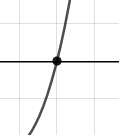
\includegraphics[width=0.3\textwidth]{../Figures/polyZeroBehaviorCopyDC.png}
    \end{center}\begin{enumerate}[label=\Alph*.]
\begin{multicols}{2}
\item 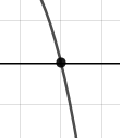
\includegraphics[width = 0.3\textwidth]{../Figures/polyZeroBehaviorCopyAC.png}
\item 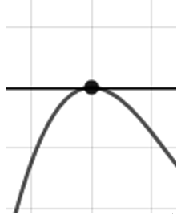
\includegraphics[width = 0.3\textwidth]{../Figures/polyZeroBehaviorCopyBC.png}
\item 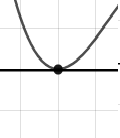
\includegraphics[width = 0.3\textwidth]{../Figures/polyZeroBehaviorCopyCC.png}
\item 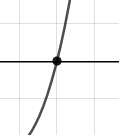
\includegraphics[width = 0.3\textwidth]{../Figures/polyZeroBehaviorCopyDC.png}
\end{multicols}\item None of the above.\end{enumerate}
\textbf{General Comment:} You will need to sketch the entire graph, then zoom in on the zero the question asks about.
}
\litem{
Which of the following equations \textit{could} be of the graph presented below?

\begin{center}
    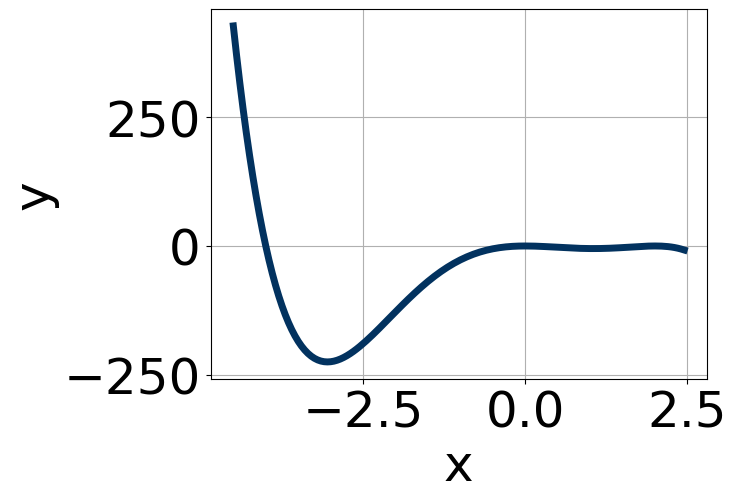
\includegraphics[width=0.5\textwidth]{../Figures/polyGraphToFunctionCopyC.png}
\end{center}


The solution is \( -20x^{4} (x - 2)^{8} (x + 4)^{11} \), which is option A.\begin{enumerate}[label=\Alph*.]
\item \( -20x^{4} (x - 2)^{8} (x + 4)^{11} \)

* This is the correct option.
\item \( -4x^{8} (x - 2)^{11} (x + 4)^{7} \)

The factor $(x - 2)$ should have an even power.
\item \( 6x^{4} (x - 2)^{6} (x + 4)^{8} \)

The factor $(x + 4)$ should have an odd power and the leading coefficient should be the opposite sign.
\item \( -7x^{8} (x - 2)^{5} (x + 4)^{8} \)

The factor $(x - 2)$ should have an even power and the factor $(x + 4)$ should have an odd power.
\item \( 14x^{6} (x - 2)^{10} (x + 4)^{7} \)

This corresponds to the leading coefficient being the opposite value than it should be.
\end{enumerate}

\textbf{General Comment:} General Comments: Draw the x-axis to determine which zeros are touching (and so have even multiplicity) or cross (and have odd multiplicity).
}
\litem{
Construct the lowest-degree polynomial given the zeros below. Then, choose the intervals that contain the coefficients of the polynomial in the form $x^3+bx^2+cx+d$.
\[ -5 - 3 i \text{ and } -2 \]The solution is \( x^{3} +12 x^{2} +54 x + 68 \), which is option D.\begin{enumerate}[label=\Alph*.]
\item \( b \in [-1, 10], c \in [6.99, 8.99], \text{ and } d \in [7, 12] \)

$x^{3} + x^{2} +7 x + 10$, which corresponds to multiplying out $(x + 5)(x + 2)$.
\item \( b \in [-16, -10], c \in [53.47, 55.02], \text{ and } d \in [-72, -63] \)

$x^{3} -12 x^{2} +54 x -68$, which corresponds to multiplying out $(x-(-5 - 3 i))(x-(-5 + 3 i))(x -2)$.
\item \( b \in [-1, 10], c \in [4.6, 5.04], \text{ and } d \in [1, 7] \)

$x^{3} + x^{2} +5 x + 6$, which corresponds to multiplying out $(x + 3)(x + 2)$.
\item \( b \in [11, 13], c \in [53.47, 55.02], \text{ and } d \in [68, 69] \)

* $x^{3} +12 x^{2} +54 x + 68$, which is the correct option.
\item \( \text{None of the above.} \)

This corresponds to making an unanticipated error or not understanding how to use nonreal complex numbers to create the lowest-degree polynomial. If you chose this and are not sure what you did wrong, please contact the coordinator for help.
\end{enumerate}

\textbf{General Comment:} Remember that the conjugate of $a+bi$ is $a-bi$. Since these zeros always come in pairs, we need to multiply out $(x-(-5 - 3 i))(x-(-5 + 3 i))(x-(-2))$.
}
\litem{
Which of the following equations \textit{could} be of the graph presented below?

\begin{center}
    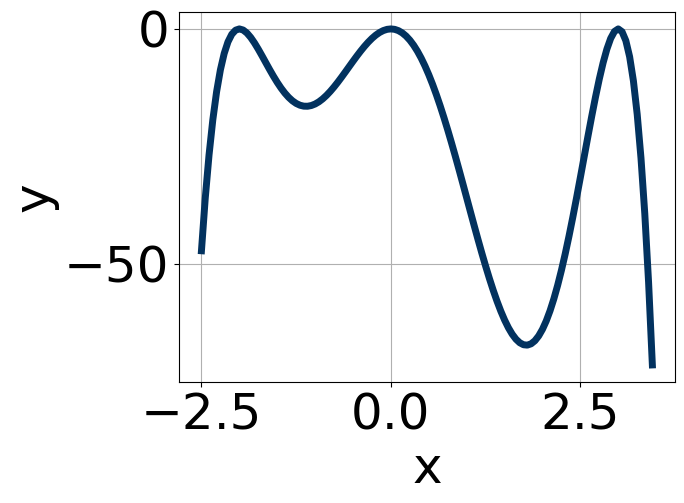
\includegraphics[width=0.5\textwidth]{../Figures/polyGraphToFunctionC.png}
\end{center}


The solution is \( -17x^{4} (x - 3)^{10} (x + 2)^{4} \), which is option C.\begin{enumerate}[label=\Alph*.]
\item \( -13x^{10} (x - 3)^{4} (x + 2)^{11} \)

The factor $(x + 2)$ should have an even power.
\item \( 11x^{4} (x - 3)^{4} (x + 2)^{4} \)

This corresponds to the leading coefficient being the opposite value than it should be.
\item \( -17x^{4} (x - 3)^{10} (x + 2)^{4} \)

* This is the correct option.
\item \( -8x^{8} (x - 3)^{7} (x + 2)^{7} \)

The factors $(x - 3)$ and $(x + 2)$ should both have even powers.
\item \( 12x^{10} (x - 3)^{10} (x + 2)^{11} \)

The factor $(x + 2)$ should have an even power and the leading coefficient should be the opposite sign.
\end{enumerate}

\textbf{General Comment:} General Comments: Draw the x-axis to determine which zeros are touching (and so have even multiplicity) or cross (and have odd multiplicity).
}
\litem{
Describe the zero behavior of the zero $x = 3$ of the polynomial below.
\[ f(x) = 5(x - 3)^{5}(x + 3)^{10}(x + 9)^{6}(x - 9)^{10} \]The solution is the graph below, which is option D.
    \begin{center}
        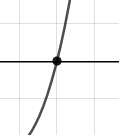
\includegraphics[width=0.3\textwidth]{../Figures/polyZeroBehaviorDC.png}
    \end{center}\begin{enumerate}[label=\Alph*.]
\begin{multicols}{2}
\item 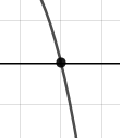
\includegraphics[width = 0.3\textwidth]{../Figures/polyZeroBehaviorAC.png}
\item 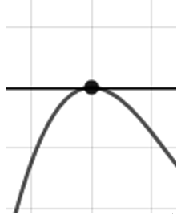
\includegraphics[width = 0.3\textwidth]{../Figures/polyZeroBehaviorBC.png}
\item 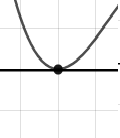
\includegraphics[width = 0.3\textwidth]{../Figures/polyZeroBehaviorCC.png}
\item 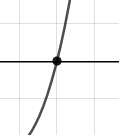
\includegraphics[width = 0.3\textwidth]{../Figures/polyZeroBehaviorDC.png}
\end{multicols}\item None of the above.\end{enumerate}
\textbf{General Comment:} You will need to sketch the entire graph, then zoom in on the zero the question asks about.
}
\litem{
Describe the end behavior of the polynomial below.
\[ f(x) = 2(x + 7)^{3}(x - 7)^{8}(x - 2)^{2}(x + 2)^{4} \]The solution is the graph below, which is option D.
    \begin{center}
        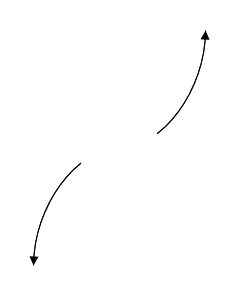
\includegraphics[width=0.3\textwidth]{../Figures/polyEndBehaviorDC.png}
    \end{center}\begin{enumerate}[label=\Alph*.]
\begin{multicols}{2}
\item 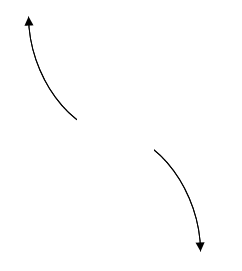
\includegraphics[width = 0.3\textwidth]{../Figures/polyEndBehaviorAC.png}
\item 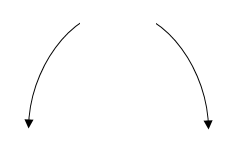
\includegraphics[width = 0.3\textwidth]{../Figures/polyEndBehaviorBC.png}
\item 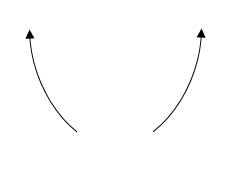
\includegraphics[width = 0.3\textwidth]{../Figures/polyEndBehaviorCC.png}
\item 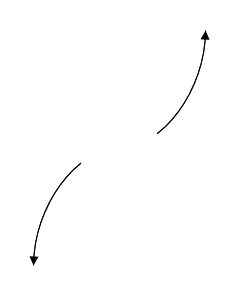
\includegraphics[width = 0.3\textwidth]{../Figures/polyEndBehaviorDC.png}
\end{multicols}\item None of the above.\end{enumerate}
\textbf{General Comment:} Remember that end behavior is determined by the leading coefficient AND whether the \textbf{sum} of the multiplicities is positive or negative.
}
\litem{
Describe the end behavior of the polynomial below.
\[ f(x) = -8(x - 9)^{4}(x + 9)^{5}(x + 2)^{4}(x - 2)^{5} \]The solution is the graph below, which is option B.
    \begin{center}
        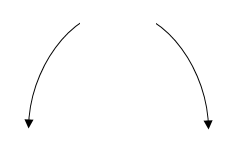
\includegraphics[width=0.3\textwidth]{../Figures/polyEndBehaviorCopyBC.png}
    \end{center}\begin{enumerate}[label=\Alph*.]
\begin{multicols}{2}
\item 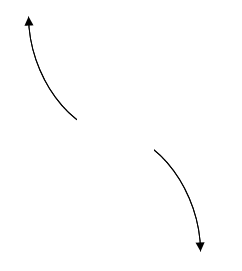
\includegraphics[width = 0.3\textwidth]{../Figures/polyEndBehaviorCopyAC.png}
\item 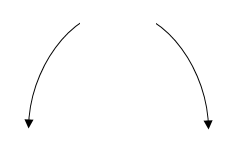
\includegraphics[width = 0.3\textwidth]{../Figures/polyEndBehaviorCopyBC.png}
\item 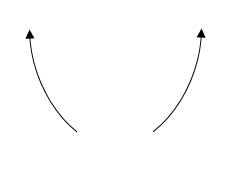
\includegraphics[width = 0.3\textwidth]{../Figures/polyEndBehaviorCopyCC.png}
\item 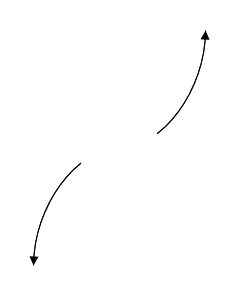
\includegraphics[width = 0.3\textwidth]{../Figures/polyEndBehaviorCopyDC.png}
\end{multicols}\item None of the above.\end{enumerate}
\textbf{General Comment:} Remember that end behavior is determined by the leading coefficient AND whether the \textbf{sum} of the multiplicities is positive or negative.
}
\litem{
Construct the lowest-degree polynomial given the zeros below. Then, choose the intervals that contain the coefficients of the polynomial in the form $ax^3+bx^2+cx+d$.
\[ \frac{-1}{4}, \frac{-1}{5}, \text{ and } \frac{4}{5} \]The solution is \( 100x^{3} -35 x^{2} -31 x -4 \), which is option D.\begin{enumerate}[label=\Alph*.]
\item \( a \in [97, 105], b \in [-39, -33], c \in [-38, -27], \text{ and } d \in [2, 6] \)

$100x^{3} -35 x^{2} -31 x + 4$, which corresponds to multiplying everything correctly except the constant term.
\item \( a \in [97, 105], b \in [-125, -121], c \in [36, 47], \text{ and } d \in [-7, -2] \)

$100x^{3} -125 x^{2} +41 x -4$, which corresponds to multiplying out $(4x -1)(5x -1)(5x -4)$.
\item \( a \in [97, 105], b \in [-87, -79], c \in [-1, 8], \text{ and } d \in [2, 6] \)

$100x^{3} -85 x^{2} -x + 4$, which corresponds to multiplying out $(4x -1)(5x + 1)(5x -4)$.
\item \( a \in [97, 105], b \in [-39, -33], c \in [-38, -27], \text{ and } d \in [-7, -2] \)

* $100x^{3} -35 x^{2} -31 x -4$, which is the correct option.
\item \( a \in [97, 105], b \in [32, 40], c \in [-38, -27], \text{ and } d \in [2, 6] \)

$100x^{3} +35 x^{2} -31 x + 4$, which corresponds to multiplying out $(4x -1)(5x -1)(5x + 4)$.
\end{enumerate}

\textbf{General Comment:} To construct the lowest-degree polynomial, you want to multiply out $(4x + 1)(5x + 1)(5x -4)$
}
\litem{
Construct the lowest-degree polynomial given the zeros below. Then, choose the intervals that contain the coefficients of the polynomial in the form $x^3+bx^2+cx+d$.
\[ 3 - 3 i \text{ and } 4 \]The solution is \( x^{3} -10 x^{2} +42 x -72 \), which is option D.\begin{enumerate}[label=\Alph*.]
\item \( b \in [-1, 7], c \in [-6, 0], \text{ and } d \in [-14, -11] \)

$x^{3} + x^{2} -x -12$, which corresponds to multiplying out $(x + 3)(x -4)$.
\item \( b \in [-1, 7], c \in [-8, -2], \text{ and } d \in [10, 13] \)

$x^{3} + x^{2} -7 x + 12$, which corresponds to multiplying out $(x -3)(x -4)$.
\item \( b \in [5, 20], c \in [34, 44], \text{ and } d \in [72, 78] \)

$x^{3} +10 x^{2} +42 x + 72$, which corresponds to multiplying out $(x-(3 - 3 i))(x-(3 + 3 i))(x + 4)$.
\item \( b \in [-10, -5], c \in [34, 44], \text{ and } d \in [-77, -69] \)

* $x^{3} -10 x^{2} +42 x -72$, which is the correct option.
\item \( \text{None of the above.} \)

This corresponds to making an unanticipated error or not understanding how to use nonreal complex numbers to create the lowest-degree polynomial. If you chose this and are not sure what you did wrong, please contact the coordinator for help.
\end{enumerate}

\textbf{General Comment:} Remember that the conjugate of $a+bi$ is $a-bi$. Since these zeros always come in pairs, we need to multiply out $(x-(3 - 3 i))(x-(3 + 3 i))(x-(4))$.
}
\end{enumerate}

\end{document}